\subsection{Coronel Blotto}

\subsubsection{Descripción del Juego}

En este juego cada uno de los jugadores tiene $S$ soldados en total que debe ubicar en $N$ campos de batallas. Cada soldado puede ser asignado a un único campo, pero cualquier número de soldados puede ser colocado en cualquier campo, incluyendo el cero. Un jugador obtiene un campo de batalla si asigna más soldados que su oponente en ese campo de batalla. El juego es ganado por el jugador que obtenga un mayor número de campos y su pago es igual a la diferencia entre el número de campos obtenidos por cada uno de los jugadores \cite{bib:introductionCFR}.

Formalmente el juego puede ser descrito de la siguiente manera. Cada jugador debe elegir $N$ números enteros, digamos $(a_1, a_2, ..., a_N)$ y $(b_1, b_2, ..., b_N)$, para el jugador $1$ y $2$ respectivamente, tales que $a_1 + a_2 + ... + a_N = S$ y $b_1 + b_2 + ... + b_N = S$, con $N < S$, donde $a_i$ y $b_i$ es la cantidad de soldados ubicados el $i$-ésimo campo por el primer y segundo jugador, respectivamente. Para estas distribuciones, la ganancia del jugador $1$ viene dada por:
\begin{alignat}{1}
|\{ 1 \leq i \leq N : a_i > b_i\}| - |\{ 1 \leq i \leq N : a_i < b_i\}|
\end{alignat}

Este juego depende de dos parámetros: el número de soldados $S$ y el número de campos de batallas $N$, por lo que la matriz de pagos no es constante y por eso no es presentada como en los juegos anteriores. La matriz para de un juego con $S$ soldados y $N$ es una matriz cuadrada de tamaño $\binom{N+S-1}{S-1}$.

\subsubsection{Detalles de Implementación}

Debido a que la descripción del juego no proporciona de forma explícita la matriz de pagos, es necesario generarla. Para esto se creó un programa que, dado el número de campos de batalla ($N$) y el número de soldados ($S$), genera todas las posibles distribuciones de cada uno de los jugadores mediante un algoritmo de \textit{backtracking} y calcula el pago para cada juego posible, obteniendo como output la matriz deseada.

\subsubsection{Resultados experimentales}

En este juego no se posee un equilibrio de Nash como referencia. Sin embargo, como la matriz de pagos es simétrica, el valor del juego debe ser $0$, así que las estrategias obtenidas, se mostradas en la Tabla \ref{tab:estrategias-coronel-blotto}, deben garantizar un valor esperado cercano a $0$. En esta tabla, también se observa que cada una de las estrategias puede garantizar un valor esperado mayor o igual que $-0.008$ en todos los casos.

\begin{table}[hbt]
    \scriptsize
    \centering
    \begin{tabular}{c}
        Estrategias \\
        \hline
        Procedimiento A \\ \hline
         $(0, 0, 0.126, 0.113, 0, 0, 0, 0.080, 0, 0.100, 0, 0.131, 0, 0.001, 0.111, 0.118, 0.094, 0.124, 0, 0, 0)$ \\
         $(0, 0, 0.101, 0.109, 0, 0, 0, 0.116, 0, 0.139, 0, 0.132, 0, 0.002, 0.076, 0.076, 0.141, 0.106, 0, 0, 0)$\\
         $(v_1, v_2) = (-0.008, -0.002)$ \\
        \hline
        Procedimiento B \\ \hline
         $(0, 0.002, 0.093, 0.110, 0.001, 0, 0.002, 0.111, 0.001, 0.128, 0.001, 0.126, 0, 0.001, 0.076, 0.112, 0.088, 0.145, 0.001, 0.001, 0)$ \\
         $(0, 0.001, 0.102, 0.107, 0.001, 0, 0.0, 0.154, 0.001, 0.099, 0, 0.055, 0.001, 0, 0.156, 0.113, 0.140, 0.069, 0.002, 0.001, 0)$ \\
         $(v_1, v_2) = (-0.007, -0.004)$ \\
        \hline
        Procedimiento C \\ \hline
         $(0, 0, 0.119, 0.106, 0, 0, 0, 0.110, 0, 0.107, 0, 0.108, 0, 0, 0.122, 0.122, 0.117, 0.1, 0, 0, 0)$ \\
         $(0, 0, 0.148, 0.096, 0, 0, 0, 0.099, 0, 0.095, 0, 0.093, 0, 0, 0.155, 0.126, 0.117, 0.070, 0, 0, 0)$ \\
         $(v_1, v_2) = (-0.005, -0.004)$ \\
        \hline
    \end{tabular}
    \caption{Estrategias obtenidas del juego Coronel Blotto}
    \label{tab:estrategias-coronel-blotto}
\end{table}

Los resultados obtenidos relacionados al tiempo y número de iteraciones de cada procedimiento son mostrados en la Tabla \ref{tab:resultados-coronel-blotto}. El procedimiento A, regret condicional, tuvo una duración promedio de $875.533$ segundos, con un número promedio de iteraciones de $190222305.3$, obteniendo un promedio de $4.60 {\times} 10^{-6}$ segundos por iteración. Con el procedimiento B, que utiliza un vector invariante de probabilidad, se obtuvo un tiempo, número de iteraciones y tiempo por iteración promedios de $79.358$ segundos, $66378.4$ iteraciones y $1.2 {\times} 10^{-3}$ segundos por iteración, respectivamente. Por último, el procedimiento C, regret incondicional, se obtuvo un tiempo promedio de $0.166$, el número de iteraciones promedio fue de $48613.5$, obteniendo un promedio de $3.41 {\times} 10^{-6}$ segundos por iteración.

\begin{table}[hbt]
   \scriptsize
    \centering
    \begin{tabular}{r r r | r r r | r r r}
    \multicolumn{3}{c}{A} & \multicolumn{3}{c}{B} & \multicolumn{3}{c}{C} \\ \hline
	$940.377$ & $197127165$ & $4.77 {\times} 10^{-06}$ & $90.239$ & $75420$ & $1.20 {\times} 10^{-03}$ & $0.047$ & $13559$ & $3.50 {\times} 10^{-06}$ \\
	$532.020$ & $109697363$ & $4.85 {\times} 10^{-06}$ & $74.886$ & $62704$ & $1.19 {\times} 10^{-03}$ & $0.192$ & $56383$ & $3.41 {\times} 10^{-06}$ \\
	$396.583$ & $82924728$ & $4.78 {\times} 10^{-06}$ & $56.735$ & $47416$ & $1.20 {\times} 10^{-03}$ & $0.046$ & $13664$ & $3.39 {\times} 10^{-06}$ \\
	$362.203$ & $80521418$ & $4.50 {\times} 10^{-06}$ & $41.290$ & $34596$ & $1.19 {\times} 10^{-03}$ & $0.162$ & $47742$ & $3.40 {\times} 10^{-06}$ \\
	$967.890$ & $207963652$ & $4.65 {\times} 10^{-06}$ & $69.359$ & $58123$ & $1.19 {\times} 10^{-03}$ & $0.090$ & $26547$ & $3.40 {\times} 10^{-06}$ \\
	$1016.540$ & $245737655$ & $4.14 {\times} 10^{-06}$ & $64.457$ & $53560$ & $1.20 {\times} 10^{-03}$ & $0.118$ & $34715$ & $3.41 {\times} 10^{-06}$ \\
	$553.971$ & $112170109$ & $4.94 {\times} 10^{-06}$ & $80.789$ & $67624$ & $1.19 {\times} 10^{-03}$ & $0.261$ & $76657$ & $3.40 {\times} 10^{-06}$ \\
	$966.339$ & $204832370$ & $4.72 {\times} 10^{-06}$ & $138.294$ & $115846$ & $1.19 {\times} 10^{-03}$ & $0.358$ & $105149$ & $3.40 {\times} 10^{-06}$ \\
	$1787.020$ & $384044065$ & $4.65 {\times} 10^{-06}$ & $84.924$ & $70978$ & $1.20 {\times} 10^{-03}$ & $0.121$ & $35434$ & $3.42 {\times} 10^{-06}$ \\
	$1232.380$ & $277204528$ & $4.45 {\times} 10^{-06}$ & $92.610$ & $77517$ & $1.19 {\times} 10^{-03}$ & $0.260$ & $76285$ & $3.41 {\times} 10^{-06}$ \\ \hline
	$875.533$ & $190222305.3$ & $4.60 {\times} 10^{-06}$ & $79.358$ & $66378.4$ & $1.20 {\times} 10^{-03}$ & $0.166$ & $48613.5$ & $3.41 {\times} 10^{-06}$ \\ \hline
    \end{tabular}
    \caption{Resultados del juego Coronel Blotto}
    \label{tab:resultados-coronel-blotto}
\end{table}

 La Figura \ref{fig:regret-coronel-blotto} muestra el regret incondicional con respecto al tiempo de la última corrida para los tres procedimientos. Se observa que el regret máximo tiende a cero para cada uno de los jugadores en todos los procedimientos.
 
\begin{figure}[hbt!]
\caption{Gráficas del regret con respecto al número de iteraciones del juego Coronel Blotto}
\label{fig:regret-coronel-blotto}
\centering
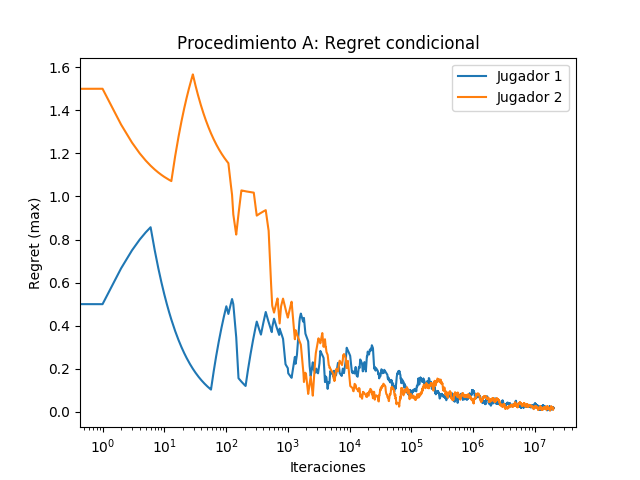
\includegraphics[width=0.45\textwidth]{graficas/coronel-blotto/procedimiento-A.png}
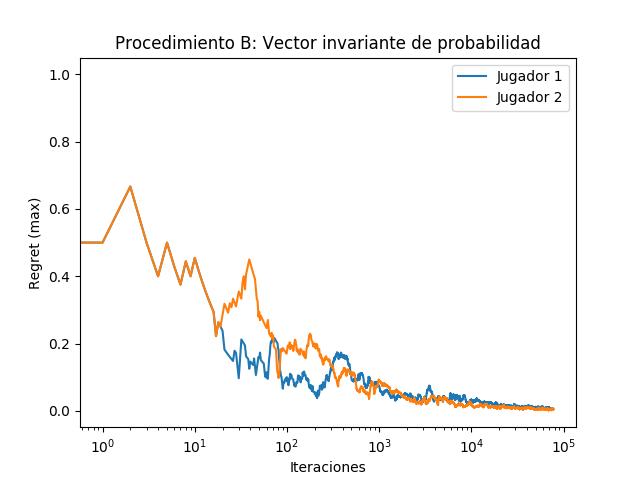
\includegraphics[width=0.45\textwidth]{graficas/coronel-blotto/procedimiento-B.png}
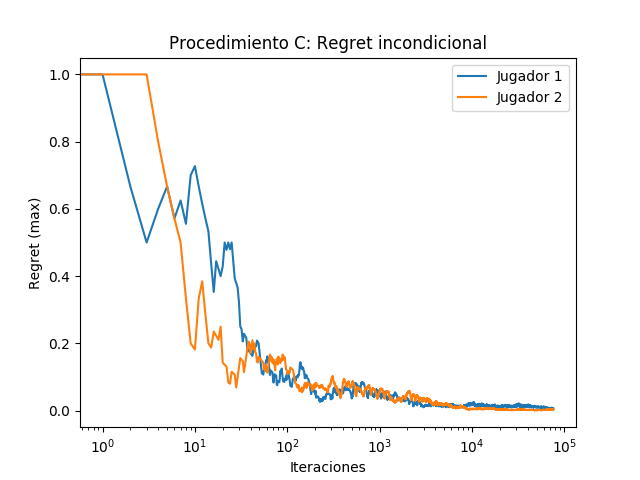
\includegraphics[width=0.45\textwidth]{graficas/coronel-blotto/procedimiento-C.png}
\end{figure}
\newpage